\section{Background}

\begin{figure*}
\centering
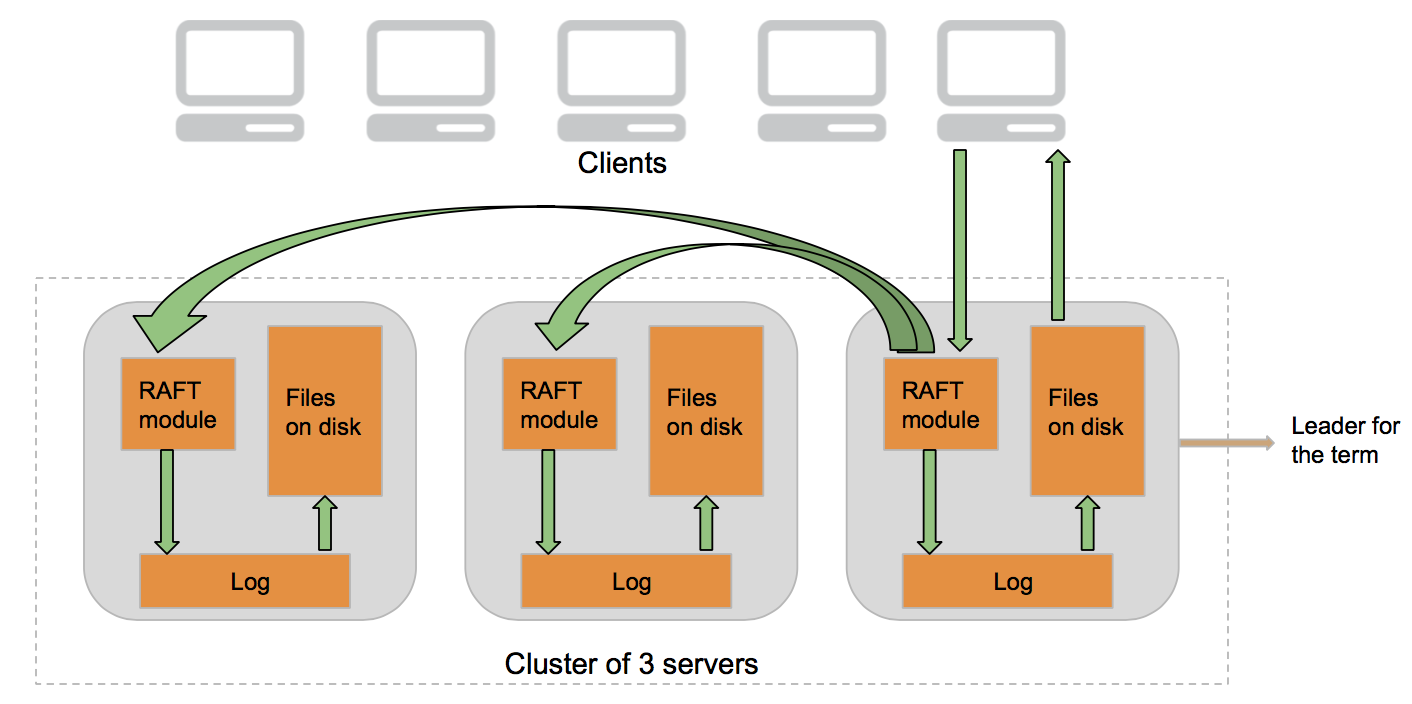
\includegraphics[height=2.3in, width=5in]{images/SystemModel.png}
\caption{Experimental setup on DigitalOcean.}~\label{fig:figure1}
\end{figure*}

Raft introduces the following significant features amongst others: strong leader; leader election and cluster membership changes. It implements consensus by first electing a leader. The protocol involves strong form of leadership in that the log entries only flow from the leader to other servers in the cluster, also known as the followers. Also, the leader never overwrites or deletes entries in its own log. This simplifies the management of replicated log and presumably makes it easier to understand the protocol. Raft divides times into terms and each term begins with leader election. It uses randomized timers to elect leader so as to resolve any conflicts. In practice, it works without having extra overhead of consensus agreement on leader. The servers in the cluster communicate using remote procedure calls(RPCs).

Write requests under normal operation works as follows : Once a leader has been elected, it begins servicing client requests. Each client request contains a command to be executed by the replicated state machines. The leader appends the command to its log as a new entry, then issues RPCs in parallel to each of the other servers to replicate the entry. When the entry has been safely replicated on a majority of servers, the leader applies the entry to its state machine and returns the result of that execution to the client. 

Read only requests can be handled without writing anything to the log. However, before responding to read request, leader ensures that it is still the leader of the cluster. Raft handles this by having the leader exchange heartbeat messages with a majority of the cluster before responding to read-only requests.

Our performance evaluation is measured in terms of read and write request time taken by the client, under various workload scenarios. It is also important to note that all requests are serviced by the leader alone. The leader taken in requests from the client and replicates log entries across the cluster. Once an entry is applied to the state machine, no other server can apply a different command for the same log index. This ensures necessary safety in the protocol. Also, clients do not maintain any active information on who the current leader of the cluster is. Thus, there is a need for client communication protocol to resolve leader id and then direct the requests to this id. 
